\chapter{Transfer Learning}
  % Brief introduction
  \lettrine[lines=2]{T}he key insight behind the idea of the transfer of knowledge comes from psychology: human beings
  learn a new task much faster if, in the past, they solved other similar tasks. Learning to drive
  a bike may facilitate learning to drive a car, learning to play organ may help in learning to play piano.\newline
  In the last years, data mining and machine learning techniques have achieved
  significant success in many knowledge-engineering areas such as classification, regression and clustering.\newline
  However, a large part of this techniques is based on the assumption that the training data
  and the test data come from the same distribution (ie. from the same task). The problem is that
  every time there is a significant difference between the two distribution the entire model
  must be learned again from scratch. In many real-world application it is impossible, every time the
  target task changes, to recollect all the needed data to train the new model. It would be nice
  to reutilize the knowledge (ie. data) collected for tasks similar to the target one.\newline
  A typical situation is when the data at hand may be easily outdated. In this case, the
  data collected at the begin of a period may not follow the same distribution at the end of the
  same period. Transfer learning may help in avoiding the effort of rebuilding the model every time.\newline
  Another field of application of transfer learning that has been deeply investigated in the last years is Reinforcement Learning.
  In this situation, the need of an efficient transfer of knowledge is even more evident. In many real-world scenario,
  (such as Robotics or applications involving human interaction) the amount time needed to learn a good policy from
  samples coming from the target tasks if often prohibitive.\newline

  \begin{figure}
    \centering
    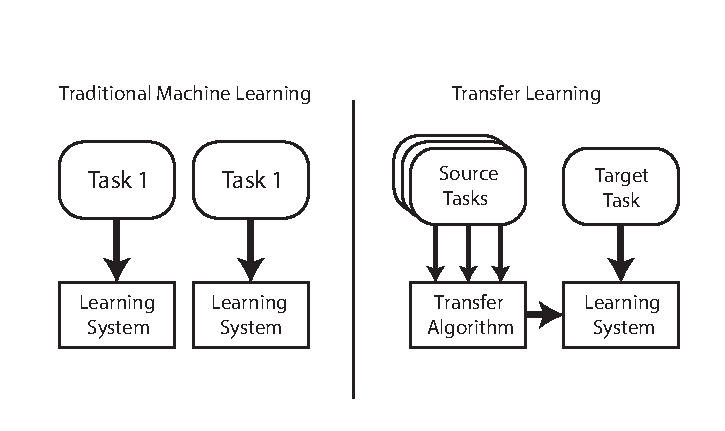
\includegraphics{images/transfervsml.pdf}
    \caption{Transfer Learning vs Traditional ML}
    \label{fig:transfertraditional}
  \end{figure}

  \noindent Transfer learning tries to reduce the learning time of an optimal policy by \textit{reusing} knowledge coming from
  previously solved task (Figure ~\ref{fig:transfertraditional}).\newline



  \section{History and Related Works}
    \noindent Scientific research on transfer learning has attracted more and more attention since 1995.\newline
    Earlier works focus on supervised learning mainly with application in classification and regression problems.
    For example~\cite{liao2005logistic} analyzes the problem of the transfer of knowledge under
    classification settings where the test and training distribution are mismatched. The authors
    propose a solution in which an auxiliary variable $\mu_i$ (for each sample $(\mathbf{x}_i^{a}, y_i^{a})$ in the training dataset)
    is introduced to reflect the mismatch between the two distributions; when $(\mathbf{x}_i^{a}, y_i^{a})$ is too
    different with respect the test distribution an appropriate choice of $\mu_i$ makes the final classifier
    less sensitive to the i$-th$ sample.\newline
    Another example, but applied to regression problems, can be found in~\cite{pardoe2010boosting}; here the authors
    try to develop one of the first general framework for transfer learning and analyze its correctness
    using the \textit{Probably Approximately Correct (PAC)} learning theory. The paper proposes a modification of the classical
    boosting algorithm to successfully include samples coming from a mismatched distribution; the goal is to learn a high
    quality model using as much as possible samples coming from the auxiliary data source.\newline
    A more theoretical work is proposed by~\cite{hanneke2013theory}; the authors explore
    a classification setting in which targets concepts are assumed to be drawn from a known
    distribution. The main goal was to study the total number of sample required to learn all targets to an
    arbitrary specified expected accuracy. The paper shows an interesting connection with the theory of
    active learning that will be discussed in the next chapter.\newline

    \noindent Only in the last 10 years research on transfer learning has focused also on reinforcement learning.
    Works that have been published differ in the type of knowledge transferred (instances, models representation or parameters)
    or in the number and domain of source and target tasks. In this thesis we mainly focus on the transfer of instances
    from a set of source tasks to a single target task; considering this setting some interesting results are presented
    in~\cite{lazaric2008transfer} where the authors successfully show (empirically) that when the samples coming from the
    source tasks are sufficiently \textit{symilar} to ones already collected for the target task, the transfer
    of instances is possible and permits to significantly reduce the time needed to learn an optimal
    policy on the target task.\newline
    A more theory-oriented work appears in~\cite{lazaric2011multiple}, this paper represents one of the
    first attempt to provide a theoretical formalization of the sample-transfer problem, in particular
    the authors provide a series of theoretical bounds for different transfer algorithm showing the potential
    of knowledge transfer in a single-task learning setting.

  \section{Taxonomy}
    \noindent In this section, inspired by~\cite{lazaric2012transfer}, we report a general classification of
    transfer learning based on: the setting, the transferred knowledge and the objective.
    \subsection{Settings}
      \noindent The settings regards the specification of the state-action domain for the tasks involved in
      the transfer. We can have three different cases:
      \begin{itemize}
        \item \textbf{Transfer from a single source task to a target task with fixed domain}. This
        setting (single source and target task) is often referred in literature as \textit{inductive transfer learning}.
        In this particular situation, we assume that both the source and the target task share the same domain, ie.
        the same state-action space. The transfer algorithm might or might not have access to the target task knowledge
        during the transfer. In the case, no knowledge from the task is available the algorithm can only
        perform a very simple transfer (without regarding the problem of the negative transfer) and directly use
        this knowledge in the target task. On the other hand if some knowledge is available from the target
        task than a more complex transfer can happen: the algorithm can adapt the knowledge of the source
        to the knowledge already present in the target, for example by only selecting, in the source task,
        those samples that are likely to be generated by the model of the target task.

        \item \textbf{Transfer across multiple tasks with fixed domain}. In this scenario we assume that many source tasks are
        available. Again, also in this case, all the tasks involved (target and sources) share the same state-action space.
        We expect that, as the number of source task increases, the performance of the target task to be much
        better compared with the previous case.

        \item \textbf{Transfer across multiple tasks with different domains}. This case represents the most general
        situation: multiple tasks are available and each task has a different state-action domain. In this scenario,
        to manage the complexity of the problem, many of the proposed algorithms reduces to the case with a single
        source and target task with different domains and focuses on the problem of defining an efficient mapping
        between the domains of the source and target task.
      \end{itemize}

    \subsection{Knowledge}
      \noindent In every transfer learning algorithm, a central problem is how to define how knowledge is
      actually used to transfer information from the source task to the target task. A possible
      categorization proposed by~\cite{lazaric2012transfer} classify the possible knowledge transfer
      approaches in: instance transfer, representation transfer and parameter transfer:
      \begin{itemize}
        \item \textbf{Instance transfer}. In this scenario, the transferred knowledge assumes the shape of
        samples of trajectories collected in the source tasks. Each sample can be viewed as a tuple
        of four elements: the staring state $s$, the action taken in $a$, the next state $s'$ reached
        after applying $a$ to $s$ and the relevant reward $r$. The transferred samples can now be used
        in the target task, in a model-free approach, for example, to build an accurate approximation
        of the value function of each state.

        \item \textbf{Representation transfer}. The idea is that each RL algorithm uses a specific
        representation of the task and of its solution. After the source tasks have learned an accurate
        solution, the transfer algorithm tries to abstract the different task-solution representations
        to permit the target task to take advantage of them. Examples range from the use of reward
        shaping functions to MDP augmentation through options.

        \item \textbf{Parameter transfer}. Every RL algorithm is characterized by a series of parameters
        that define its own initialization. The key idea is that a good initialization can provide
        a big advantage, in terms of time to convergence, to the RL algorithm running over the target task.
        Examples can be the initial Q values for a Q-Learning algorithm or the learning rate $\alpha$ for a
        more generic algorithm. In some other situation it may be useful to adapt and change the parameters
        according to the target task.
      \end{itemize}

    \subsection{Objectives}
      \noindent It happens often in machine learning (especially in unsupervised settings) to have difficulty
      in measuring the quality of the results. This is true also in transfer learning where several metrics have been defined:
      \begin{itemize}
        \item \textbf{Learning speed improvement}. Here the objective is to measure the gain of the transfer algorithm
        in terms of amount of experience needed to learn the target task. The complexity is then measured in terms
        of samples needed to learn the optimal policy, often referred in literature (especially in supervised learning
        settings) as sample complexity. This type of objective is common when the algorithm is based on the transfer of
        instances. In practice three different metrics are commonly used: \textit{time to threshold}, \textit{area ratio}
        and \textit{finite-sample analysis}. Time to threshold measures how much experience (ie. samples) are needed to
        the algorithm to reach a fixed threshold, the main disadvantage is that the threshold may be arbitrarily chosen
        and bad representing the real situation. The area ratio is formally defined as the ratio between the learning
        curve with and without transfer, precisely:
        \begin{equation*}
          r = \frac{\text{area with transfer} - \text{area without transfer}}{\text{area without transfer}}
        \end{equation*}
        while this metrics does not suffer from the disadvantage previously described, it is scale dependent; that is
        it depends on the unit of measure of the learning curve.\newline
        The last metric represents a more theoretical approach: the idea is to derive bounds that strictly
        depend on the algorithm used, the number of samples available from the source task and the initialization
        parameters of the algorithm itself.

        \item \textbf{Asymptotic improvement}. In the major part of the applications of transfer algorithms, obtaining
        an optimal solution over the target task is often infeasible. In this situation, usually, we are interested
        in getting the solution that asymptotically achieves the best performances.
        This type of objective is usually targeted by representation transfer
        algorithm where the structure of the hypothesis space is transformed so to accurately approximate the solution
        of the target task. Up to date no transfer learning algorithm is guaranteed to improve the average approximation
        error with respect to a non-transfer algorithm.

        \item \textbf{Jumpstart improvement}. This type of objective is usually targeted by parameters transfer
        algorithms. As already mentioned above the performance of any reinforcement learning algorithm strongly
        depends on the initialization of the parameters. A bad initialization often negatively bias the target task
        and leads to longer times of convergence. Common ways to measure this type of improvements are often related
        to the comparison of the performance of the algorithm, in one case initialized with a suitable hypothesis and
        in another randomly initialized.
      \end{itemize}

      \section{Bias-Variance tradeoff}
      	\noindent In this section, we revise the theory behind of the bias-variance tradeoff. This concept represents a key idea in a
      	general machine learning framework and plays a central role in this thesis.
      	For this discussion we do not focus only on the reinforcement learning framework given that this concept is much more general.\newline

      	\noindent The idea behind the bias-variance dilemma is that for any machine learning algorithm the prediction error can
      	always be decomposed in the sum of three components:
      	\begin{equation*}
      		Total Error = Irreducible Error + Bias + Variance
      	\end{equation*}
      	The irreducible error, as the term suggest, can not be reduced regardless the algorithm used. It is the error
      	introduced from the particular realization of the training dataset $\mathcal{D}$, it represents the intrinsic error present in the data.\newline
      	Assume $\mathcal{H}$ to be the space of all the possible concepts (id. functions, also referred as hypothesis) learnable by any machine learning algorithm.
      	Suppose to fix a precise algorithm $\mathcal{A}$ and indicated with $\mathcal{C} \subset \mathcal{H}$ the set of concepts algorithm $\mathcal{A}$ can produce
      	as output. The true model (ie. the concepts that we are trying to learn) $\hat{f}$ might be inside or outside $\mathcal{C}$. On the basis of the samples
      	inside the dataset we can estimate an error function $L$ that, given an hypothesis, it returns the generalization error. We indicate as $\bar{f}$ the
      	concept learnt by $\mathcal{A}$ by minimizing $L$.\newline
      	The situation is summarized by figure~\ref{fig:biasvariance}\newline

      	\noindent The \textbf{bias} can be seen as the distance between the hypothesis learnt by $\mathcal{A}$ and the true concept $\hat{f}$. On the
      	other side the \textbf{variance} can be seen as the difference between what the algorithm has learnt from a particular
      	dataset and what the algorithm expect to learn.\newline
      	Consider the case where we have a perfect estimation of $L$ (ie. when the dataset $\mathcal{D}$ contains an infinite number of samples);
      	in this case we have an extremely low variance while the bias depends wether $\hat{f}$ is inside or outside $\mathcal{C}$.\newline
      	Suppose now that $\mathcal{D}$ contains a limited number of samples, then the estimation of $L$ will not be perfect but it will depend on
      	the number of samples available and on the complexity of $\mathcal{A}$; the higher the complexity of the model and the lower the number of samples
      	the higher the variance (\textit{overfitting}). The smaller the complexity of the model the higher the bias (\textit{underfitting}). The idea is
      	summarized in figure~\ref{fig:biasvariancegraph}.

      	\begin{figure}[!tbp]
      	  \centering
      	  \begin{minipage}[b]{0.4\textwidth}
      	    \includegraphics[scale=0.55]{images/biasvariance.eps}
      	    \caption{The hypothesis space $\mathcal{H}$, the true function $f$ and the error function (color gradient) }
      			\label{fig:biasvariance}
      	  \end{minipage}
      	  \hfill
      	  \begin{minipage}[b]{0.5\textwidth}
      	    \includegraphics[scale=0.55]{images/biasvariancegraph.eps}
      	    \caption{The graph shows the relationship between bias,variance and total error with respect to the model complexity}
      			\label{fig:biasvariancegraph}
      	  \end{minipage}
      	\end{figure}


      	\noindent The \textit{dilemma} consists in managing the complexity of the model, the power of the model and the number of samples in the
      	dataset to reach a situation where both variance and bias are close to zero, that is minimize as much as possible the total error
      	of the model.

      	\noindent As already highlighted the bias-variance dilemma is fundamental importance also in the context of transfer learning.
      	When samples are transferred from a source task to a target task we are introducing a bias in the learning performance
      	of the target, but at the same time, given that more samples are available for the learning algorithm, we are reducing
      	the variance of the estimation. The objective of the next chapters will be to seek the optimal tradeoff between the
      	bias increase and variance reduction.

        \section{Formal specification and Assumptions}
          \noindent In the following we provide the notation used in the rest of the work.
          \begin{definition}
            A task $T$ is an MDP defined as a tuple $(\mathcal{S},\mathcal{A},\mathcal{P}_T,\mathcal{R}_T,\gamma)$.
          \end{definition}

          \noindent In our situation we have a set of source MDPs plus a target MDP: $\mathcal{M}_1,\mathcal{M}_2, \dots, \mathcal{M}_n$
          where $\mathcal{M}_1, \dots, \mathcal{M}_{n-1}$ are the source MDPs and $\mathcal{M}_n$ is the target MDP.\newline
          In our framework we focus on the transfer of samples between the source MDPs and the target MDP; a
          sample in our context is a tuple $(s,a,s^{'},r)$ where $s$ and $s^{'}$ are states, $a$ is an action and $r$ is the reward associated with the transition $s,a,s'$.\newline
          We also assume that all the tasks (target included) share the same state-action space, so that no mappings are needed
          to transfer the samples.\newline

          \noindent Precisely we suppose that a number $N_t$ of samples are available
          from the target task and $N_s$ total samples are available from all the target task, with $N_t << N_s$.\newline
          Moreover, as already stated, a transfer algorithm cannot blindly transfer all the samples to the target
          task due to the possibility of a negative transfer; indeed samples coming from the target task bring a certain
          amount of variance reduction and are unbiased while samples coming from the source tasks still bring to a reduction
          over the variance but they are biased given that they come from a task that a priori might be very different
          from the target task. Therefore when transferring samples from the source tasks an estimation of the bias must be available
          and more precisely we say that the transfer is positive when the increment of the bias is lower than the decrement of the variance.
          In our case we provide a way to minimize the bias introduced by the transferred samples.
